\ifx\boi\undefined\ifx\problemname\undefined
\providecommand\sampleinputname{}
\providecommand\sampleoutputname{}
\documentclass[english]{templates/boi}
\problemlanguage{.en}
\fi
\newcommand{\boi}{Baltic Olympiad in Informatics}
\newcommand{\practicesession}{Practice Session}
\newcommand{\contestdates}{April 27 - May 1, 2018}
\newcommand{\dayone}{Day 1}
\newcommand{\daytwo}{Day 2}
\newcommand{\licensingtext}{This problem is licensed under CC BY-SA 4.0.}
\newcommand{\problem}{Problem}
\newcommand{\inputsection}{Input}
\newcommand{\outputsection}{Output}
\newcommand{\interactivity}{Interactivity}
\newcommand{\grading}{Grading}
\newcommand{\scoring}{Scoring}
\newcommand{\constraints}{Constraints}
\renewcommand{\sampleinputname}{Sample Input}
\renewcommand{\sampleoutputname}{Sample Output}
\newcommand{\sampleexplanation}[1]{Explanation of Sample #1}
\newcommand{\sampleexplanations}{Explanation of Samples}
\newcommand{\timelimit}{Time Limit}
\newcommand{\memorylimit}{Memory Limit}
\newcommand{\seconds}{s}
\newcommand{\megabytes}{MB}
\newcommand{\group}{Group}
\newcommand{\points}{Points}
\newcommand{\limitsname}{Limits}
\newcommand{\additionalconstraints}{Additional Constraints}
\newcommand{\testgroups}{
Your solution will be tested on a set of test groups, each worth a number of points.
Each test group contains a set of test cases.
To get the points for a test group you need to solve all test cases in the test group.
Your final score will be the maximum score of a single submission.
}
\fi
\def\version{jury-1}
\problemname{Vahelduvvool}
Fredrik mängib kodus iseehitatud mudelraudteega, mille üle ta on väga uhke.
Raudtee koosneb $N$ lõigust, mis on ühendatud ringiks ja nummerdatud päripäeva $1, 2, \dots, N$.
Rong saab elektrivoolu $M$ juhtmekaare kaudu, mis on paigutatud piki raudteed. Iga raudteelõik on kaetud vähemalt ühe juhtmekaarega.

Fredrik on aga ringiratast sõitvast rongist tüdinud ja otsustab iga lõigu juurde lisada \emph{raudteepöörme}, mida ta saaks kasutada rongide raudteelt maha juhtimiseks. Pöörmed nõuavad samuti elektrivoolu, täpsemalt vahelduvvoolu. \footnote{Seda sellepärast, et rootsi keeles on raudteepööre (``växlar'') ja vahelduvvool (``växelström'').}

Fredrik arvab, et vahelduvvoolu saab, kui elektrivool saab minna mõlemas suunas.
Igas juhtmes saab vool minna ainult ühes Fredriku valitud suunas (päripäeva või vastupäeva).
Seega tahab ta määrata iga juhtme elektrivoolu suuna nii, et iga raudteelõik
oleks kaetud nii päripäeva liikuva elektrivooluga juhtmega kui ka vastupäeva vooluga juhtmega.

Kas saad Fredrikut aidata?

\vspace{2mm}
%\hspace*{2mm}
\begin{center}
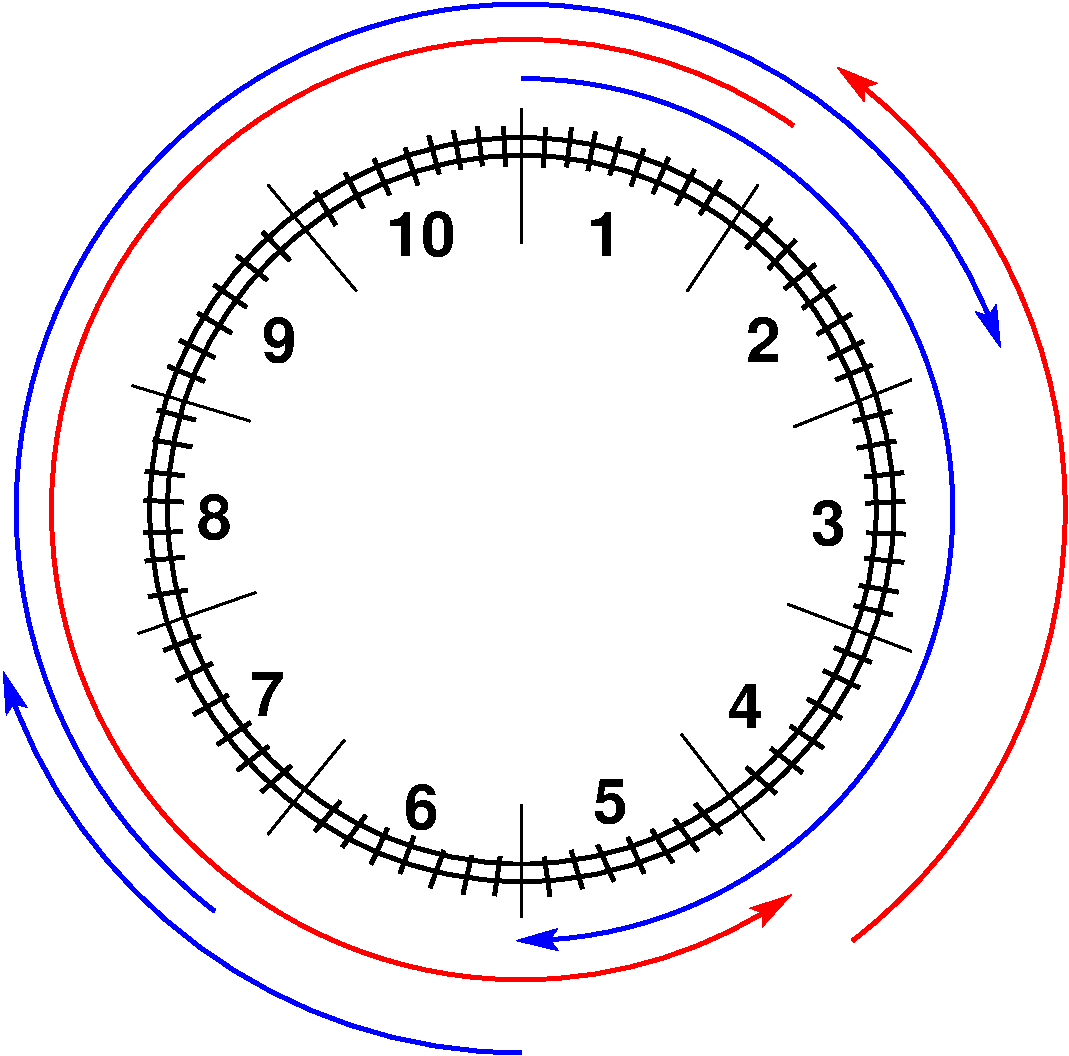
\includegraphics[width=0.5\textwidth]{alternatingfig.pdf}
\end{center}
\vspace{1mm}
{\em Esimese näite lahendus. Nooled raudteest väljaspool tähistavad elektrivooluga juhtmekaari. Iga noole suund näitab voolu suunda (sinised ja punased nooled näitavad eri suundasid). Paneme tähele, et kõigi noolte ümberpööramisel saame teise õige lahenduse: \texttt{11010}.}

\section*{\inputsection}

Esimesel real on kaks täisarvu $N$ ja $M$, vastavalt raudteelõikude arv ja juhtmekaarte arv.

Järgmisel $M$ real on igaühel kaks arvu $1 \le a, b \le N$, mis näitavad, et lõike $a, a+1, \dots, b$ katab üks juhe.
Kui $b$ on väiksem kui $a$, tähendab see, et kaar läheb üle $N$ ja $1$ ühenduskoha, st lõigud $a, \dots, N, 1, \dots, b$ on juhtme poolt kaetud.
Paneme tähele, et kui $a=b$, siis katab kaar ainult üht lõiku.

\section*{\outputsection}
Väljundisse kirjutada üks rida $M$ tähemärgiga, millest igaüks on \texttt{0} või \texttt{1}.
Tähemärk number $i$ peaks olema \texttt{0}, kui sisendi kaar number $i$ peaks olema päripäeva elektrivooluga
ja \texttt{1}, kui kaar peaks olema vastupäeva vooluga.
Kui leidub mitu lahendust, väljastada ükskõik milline neist.

Kui kaartele pole võimalik vajalikul viisil suundasid anda, väljastada ``\texttt{impossible}''.

\section*{\constraints}
\testgroups

\noindent
\begin{tabular}{| l | l | l | l |}
\hline
\textbf{\group} & \textbf{\points} & \textbf{\limitsname} & \textbf{\additionalconstraints} \\ \hline
  1     & 13     & $2 \le N, M \le 15$ & \\ \hline
  2     & 20     & $2 \le N, M \le 100$ & \\ \hline
  3     & 22     & $2 \le N, M \le 1000$ & \\ \hline
  4     & 19     & $2 \le N, M \le 100\,000$ & Ühegi kaare puhul ei ole $b < a$. \\ \hline
  5     & 26     & $2 \le N, M \le 100\,000$ & \\ \hline
\end{tabular}

